\documentclass[11pt, oneside]{article} 
\usepackage{geometry}
\geometry{letterpaper} 
\usepackage{graphicx}
	
\usepackage{amssymb}
\usepackage{amsmath}
\usepackage{parskip}
\usepackage{color}
\usepackage{hyperref}

\graphicspath{{/Users/telliott_admin/Dropbox/Tex/png/}}
% \begin{center} 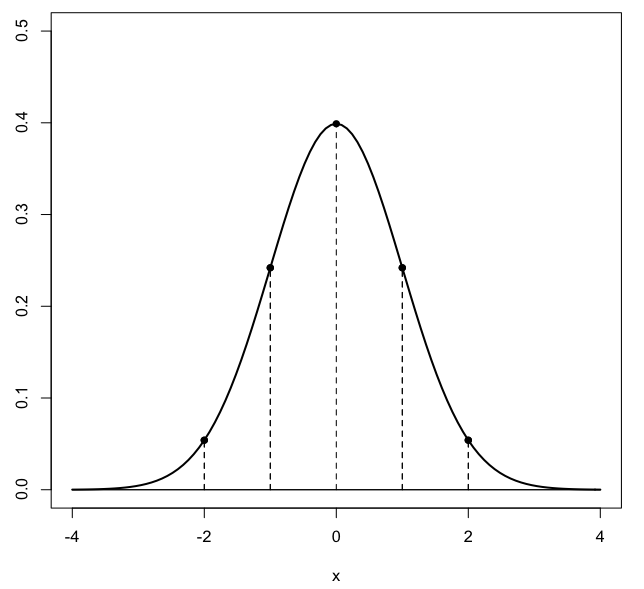
\includegraphics [scale=0.4] {gauss3.png} \end{center}

\title{Jacobian}
\date{}

\begin{document}
\maketitle
\Large

In the previous chapter, we saw that the area element in polar coordinates is
\[ r \ dr \ d \theta \]

and the volume element in spherical coordinates is
\[ dV = \rho^2 \sin \phi  \ d \rho \ d \phi \ d \theta \]
We want to develop this in a more systematic way.

\subsection*{Ellipse}
Let's think about a standard ellipse
\[ \frac{x^2}{a^2} + \frac{y^2}{b^2} = 1 \]
Following the examples in the previous chapter, we might think about trying to compute the area of this ellipse as follows
\[ A = \iint\limits_{R} 1 \ dA = \iint\limits_{R} 1 \ dx \ dy \]
The problem is that we do not know how to specify the region for an ellipse, at least, not simply.  

However, a little trick can make that problem go away!

We will change both the horizontal and vertical dimensions by constant factors (different for $x$ and $y$).  We compress --- well, the opposite of stretching --- $x$ by the factor $1/a$ and similarly compress $y$ by the factor $1/b$.  We do this by making a change of variables
\[ x = au\] 
\[ dx = a\ du \]

\[ y = bv \]
\[ dy = b\ dv \]
So 
\[ dx \ dy = ab \ du \ dv \]
Substituting
\[ \frac{(au)^2}{a^2} + \frac{(bv)^2}{b^2} = u^2 + v^2 = 1\]
The substitution has converted the ellipse into a circle of radius $1$ and area $A = \pi$.
and
\[ A = \iint\limits_{R} 1 \ dx \ dy =  \iint\limits_{R} ab \ du \ dv \]
\[ = ab \iint\limits_{R} 1 \ du \ dv \]
Now, we know the area of the region in $u,v$ coordinates, it is a circle of radius $1$ and its area is just equal to $\pi$.  So finally
\[ A = ab \iint\limits_{R} 1 \ du \ dv = \pi a b \]

This is a really simple, beautiful result.  The two copies of $r$ in the formula $A= \pi r^2$ become $a \times b$.  Both dimensions make equivalent contributions to the area, as we'd expect.

The more formal way to do this is to compute what's called the Jacobian.  It gives the ratio between areas determined in two different coordinate systems.  We take the partial derivatives of $x$ with respect to $u$ and $v$, and similarly for $y$.
\[ x_u = a \]
\[ x_v = 0 \]
\[ y_u = 0 \]
\[ y_v = b \]

The two partials ($x_v$ and $y_u$) are zero because $x$ does not depend on $v$ and  $y$ does not depend on $u$.

We evaluate the determinant of this matrix:
\[ J = 
\begin{vmatrix}
x_u & x_v \\
y_u & y_v 
\end{vmatrix} =
\begin{vmatrix}
a & 0 \\
0 & b
\end{vmatrix} =ab
\]
If necessary, we take its absolute value.  And that's the factor for converting between the two coordinate systems.

Sometimes the Jacobian is written as
\[ J = 
\begin{vmatrix}
x_u & y_u \\
x_v & y_v 
\end{vmatrix}
\]
but this doesn't change anything, because $det(A) = det(A^T)$.

To summarize:
\[ dx \ dy = J \ du \ dv \]
where
$J$ is computed as described.

\section*{Circle}
The Jacobian is done like this: 
\[ x = r \cos \theta \]
\[ y = r \sin\ \theta \]

We compute
\[ x_r = \frac{\partial x}{\partial r} = cos \ \theta \]
\[ x_{\theta} = \frac{\partial x}{\partial \theta} = -r \ sin \ \theta \]
and similarly for $y$.  Then
\[ J = 
\begin{vmatrix}
x_r & x_{\theta} \\
y_r & y_{\theta} 
\end{vmatrix} =
\begin{vmatrix}
\cos\ \theta & -r \ sin\ \theta \\
\sin\ \theta & r \ cos\ \theta 
\end{vmatrix} = r (cos^2\ \theta + sin^2\ \theta) = r
\]
This is the factor for the ratio of areas under the two systems, and that's why we have $r\ dr \ d\theta$ in the integral.  Notice that when we took the partial derivatives, they were partials of $x,y$ with respect to $r,\theta$, and we end up multiplying $dr \ d\theta$ by J.

\subsection*{General method}
Suppose we wish to determine an area by integration and we're working with the unit square $x=0 \to x=1$ and $y=0 \to y=1$, sometimes written as $[\ 0,1\ ] \times [\ 0,1\ ]$.  The area is clearly just $1$.  Now we want to make a change of variables for some reason, maybe to work on a function that's easier to deal with after the substitution, or because we have some weird bounds in our problem.
\[ u = 3x-2y \]
\[ v = x + y \]
We figure out the "exchange rate" for area by tracing out the parallelogram formed by this linear transformation

\begin{align*}
& (0,0) \to (0,0) \\
& (1,0) \to (3,1) \\
& (0,1) \to (-2,1)
\end{align*}

If we think of the vectors from $0,0$ to $(3,1)$ as $\langle 3, 1 \rangle$,  and from $0,0$ to $(-2,1)$ as $\langle -2 ,1 \rangle$, the area of the parallelogram formed by these vectors is given by the determinant
\[
| \langle 3, 1 \rangle \times \langle -2 ,1 \rangle | =
\begin{vmatrix}
3 & -2 \\
1 & \ \ 1 
\end{vmatrix} = 5
\]
The other way to do this calculation is (as we've been doing)
\[ u_x = 3 \]
\[ u_y = -2 \]
\[ v_x = 1 \]
\[ v_y = 1 \]
The Jacobian
\[ J = 
\begin{vmatrix}
u_x & u_y \\
v_x & v_y 
\end{vmatrix} = 
\begin{vmatrix}
3 & -2 \\
1 & \ \ 1 
\end{vmatrix}
= 3 - (-2) = 5 \]
Or more simply
\[ J = u_x v_y - u_y v_x = 3  - (-2) = 5 \]
And again, since we took the derivatives with respect to $x$ and $y$, we multiply $dx \ dy$ by $J$.

Each element of the area determined in $uv$ units is worth $5$ of an element in $xy$ units.
\[ 5 \iint\limits_{R}  f(x,y) \ dx \ dy = \iint\limits_{R}  f(u,v) \ du \ dv \]
\begin{equation}
\boxed{du \ dv = J \ dx \ dy }
\end{equation}

To say the above one more time in slightly different language, we have
\[ u = u(x,y) \]
\[ v = v(x,y) \]
If we change $x$ by a little bit $\Delta x$ and $y$ by a little bit $\Delta y$, by how much do $u$ and $v$ change? 
The linear approximation is
\[ \Delta u = u_x \Delta x + u_y \Delta y \]
\[ \Delta v = v_x \Delta x + v_y \Delta y \]
So for $\Delta x = 1$, the vector $<1,0>$ becomes
\[ \ <u_x ,v_x> \]
and $<0,1>$ becomes
\[ \ <u_y ,v_y> \]
and the area of the parallelogram formed by these two vectors (the area in $uv$-coordinates) is the absolute value of the cross product (think of them as lying in the plane, so there is only one term)
\[ <u_x ,v_x> \ \times  <u_y ,v_y > \]
\[ J = u_x v_y - u_y v_x \]
So for each unit $dx \ dy$ we get $du \ dv = J \ dx \ dy $ in the $uv$-coordinate system.

\subsection*{Tilted ellipse}
Here is the equation of an ellipse, although that may be hard to recognize at first.
\[ x^2 + 4xy + 13y^2 = 16 \]
If you remember (or look up) the formula
\[ Ax^2 + Bxy + Cy^2 + Dx + Ey + F = 0 \]
\[ A,B,C = 1,4,13 \]
The discriminant is
\[ B^2 - 4AC = 16 - 52 = -36 < 0 \]
Since it's $ < 0 $, this is an ellipse.  Or we could just get a plotting program like Grapher to plot it
\begin{center} 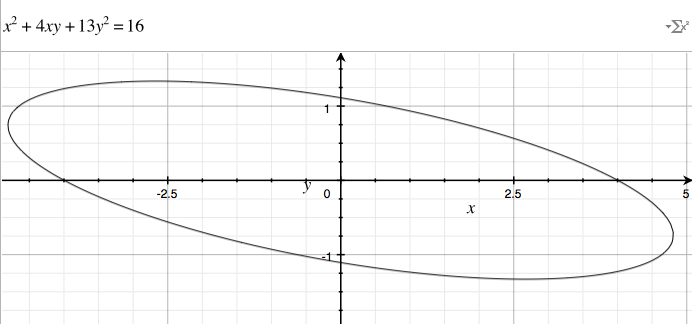
\includegraphics [scale=0.4] {tilted_ellipse.png} \end{center}

If we knew the angle of the tilt, and there is a method for that, we could rotate to a new coordinate system and just compute the area as $\pi ab$.  However, there is another way which I think is easier.  We "complete the square" to remove the term $4xy$ which "mixes" $x$ and $y$.  Since
\[ (x + 2y)^2 = x^2 + 4xy + 4y^2 \]
Our equation is transformed as follows
\[ x^2 + 4xy + 13y^2 = 16 \]
\[ \ [ \ x^2 + 4xy + 4y^2  \ ] \ + 9y^2  = 16 \]
\[ (x + 2y)^2 + 9y^2 = 16 \]
We do a substitution almost like before, but modified:
\[ u = x + 2y \]
\[ v = 3y \]
so now we have
\[ u^2 + v^2 = 16 \]
This is a circle of radius $4$ and area $16\pi$.
Now we just need the Jacobian:
\[ u_x = 1 \]
\[ u_y = 2 \]
\[ v_x = 0 \]
\[ v_y = 3 \]
\[ J = 
\begin{vmatrix}
u_x & u_y \\
v_x & v_y 
\end{vmatrix} = 
\begin{vmatrix}
1 & 2 \\
0 & 3 
\end{vmatrix}
= 3 \]
\[ du \ dv = 3 \ dx \ dy \]
When we took the partial derivatives, they were partials of $u,v$ with respect to $x,y$, so we end up multiplying $dx \ dy$ by J.
\[ \frac{1}{3} du \ dv = dx \ dy \]
We need to multiply the area by this factor to give a final answer of $16\pi/3$.

\subsection*{Varberg example}
The next example is from Varberg, 17.16.
\begin{center} 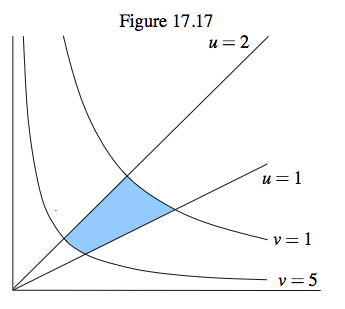
\includegraphics [scale=0.6] {Varberg-17-16.png} \end{center}
We have the lines $x=y$ and $x=2y$ and the curves $xy=1$ and $xy=5$.  Looks like $xy$ would be a good variable to have so
\[ u = \frac{x}{y} \]
\[ v = xy \]
These suggestions come from Varberg, not me.  :)  

The boundaries of the region are just $u = 1 \rightarrow u = 2$ and $v = 1 \rightarrow v = 5 $.
Rearranging:
\[ x = uy \]
\[ x = \frac{v}{y} \]
\[ x^2 = xx = uy \ \frac{v}{y} =  uv \]

For the Jacobian, it is important to solve for $x,y$ in terms of $u,v$, and not the other way around, so that we'll have terms containing $u$ and $v$ in the final integral.
\[ x = \sqrt{uv} \]
\[ y^2 = \frac{x}{u} \frac{v}{x} = \frac{v}{u} \]
\[ y = \sqrt{\frac{v}{u}} \]
So 
\[ x_u = \frac{1}{2} \sqrt{\frac{v}{u}} \]
\[ x_v =  \frac{1}{2} \sqrt{\frac{u}{v}} \]
\[ y_u =  -\frac{1}{2u} \sqrt{\frac{v}{u}}\]
\[ y_v = \frac{1}{2} \sqrt{\frac{1}{uv}} \]
The Jacobian is then
\[ x_u y_v - x_v y_u \]
\[ \frac{1}{2} \sqrt{\frac{v}{u}} \ \frac{1}{2} \sqrt{\frac{1}{uv}} + \frac{1}{2} \sqrt{\frac{u}{v}} \  \frac{1}{2u} \sqrt{\frac{v}{u}} \]
\[ = \frac{1}{4u} + \frac{1}{4u} = \frac{1}{2u} \]
The area is 
\[ A = \iint\limits_{R} 1 \ dx \ dy =  \iint\limits_{R} \frac{1}{2u}  \ du \ dv \]
\[ = \int_{u=1}^{2} \ \int_{v=1}^{5} \frac{1}{2u}  \ dv \ du \]
\[ = 2 \int_{u=1}^{2} \ \frac{1}{u} \ du = 2 \ln 2 \]

\subsection*{spherical coordinates}
In the previous chapter, we found the volume element for the sphere as
\[ dV = \rho^2 \sin \phi \ d \rho \ d \phi \ d \theta \]
by analyzing the sides of the volume element.  We can do this more formally, using the Jacobian.  It is a bit of a mess but we get there in the end.

In 2D we write
\[ x = r \cos \theta \]
\[ y = r \sin \theta \]

In 3D we write
\[ x = \rho \sin \phi \cos \theta \]
\[ y = \rho \sin \phi \sin \theta \]
\[ z = \rho \cos \phi \]
\begin{center} 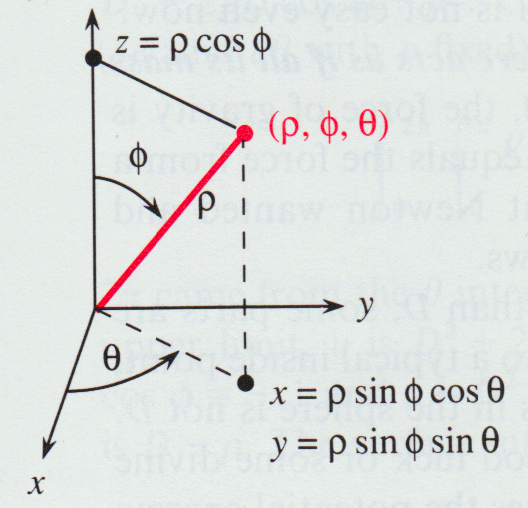
\includegraphics [scale=0.5] {spherical_coordinates2.png} \end{center}

We need to compute $9$ partial derivatives:
\[ x_{\rho} = \sin \phi \cos \theta \]
\[ x_{\phi}  = \rho \cos \phi \cos \theta \]
\[ x_{\theta} = -\rho \sin \phi \sin \theta \]

\[ y_{\rho} = \sin \phi \sin \theta \]
\[ y_{\phi}  = \rho \cos \phi \sin \theta \]
\[ y_{\theta} = \rho \sin \phi \cos \theta \]

\[ z_{\rho} = \cos \phi \]
\[ z_{\phi}  = -\rho \sin \phi \]
\[ z_{\theta} = 0 \]

Compute the determinant of this $3 \times 3$ matrix:
\[ \begin{vmatrix}
x_{\rho} = \sin \phi \cos \theta && x_{\phi}  = \rho \cos \phi \cos \theta &&x_{\theta} = -\rho \sin \phi \sin \theta  \\
y_{\rho} = \sin \phi \sin \theta && y_{\phi}  = \rho \cos \phi \sin \theta && y_{\theta} = \rho \sin \phi \cos \theta  \\
z_{\rho} = \cos \phi &&  z_{\phi}  = -\rho \sin \phi && z_{\theta} = 0
\end{vmatrix} \]

We should use the third row or the third column because $z_{\theta} = 0$.  

We choose the third row because we notice that
\[ x_{\phi} y_{\theta} = \rho \cos \phi \cos \theta \ \rho \sin \phi \cos \theta = \rho^2 \sin \phi \cos \phi \cos^2 \theta \]
\[ x_{\theta} y_{\phi} = -\rho \sin \phi \sin \theta \ \rho \cos \phi \sin \theta = -\rho^2 \sin \phi \cos \phi \sin^2 \theta \]
So subtracting, we get 
\[ \rho^2 \sin \phi \cos \phi (\cos^2 \theta + \sin^2 \theta) \]
\[ = \rho^2 \sin \phi \cos \phi \]
Multiplying by $z_\rho$ gives
\[ = \rho^2 \sin \phi \cos^2 \phi \]
which should look vaguely familiar.

For the second term of the determinant we compute
\[ x_{\rho} y_{\theta} = \sin \phi \cos \theta \ \rho \sin \phi \cos \theta  = \rho \sin^2 \phi \cos^2 \theta \]
\[ x_{\theta} y_{\rho} = -\rho \sin \phi \sin \theta \ \sin \phi \sin \theta = -\rho \sin^2 \phi \sin^2 \theta \]
So, subtracting, we get
\[ = \rho \sin^2 \phi (\cos^2 \theta + \sin^2 \theta) \]
\[ = \rho \sin^2 \phi \]
Multiplying by $z_\phi$ gives
\[ - \rho^2 \sin^3 \phi \]

Finally, subtract the second term from the first:
\[ \rho^2 \sin \phi \cos^2 \phi + \rho^2 \sin^3 \phi  = \rho^2 \sin \phi \]
Which is exactly what we said before!



\end{document}